\section{Durchführung}
\subsection{Ablenkung im elektrischen Feld}

\label{sec:Durchführung}
Vor Beginn der Messung muss die Kathodenstrahlröhre zunächst mindestens 1 Minute
geheizt werden.
Dann wird zuerst die Proportionalität zwischen Verschiebung und Spannung untersucht, indem
für fünf verschiedene Beschleunigungsspannungen $U_B$ zwischen 180 und 500 $\si{\volt}$
die Ablenkspannung so eingestellt wird, dass der Auftreffpunkt jeweils auf einer der
9 äquidistanten Linien des Schirms liegt. Die zu verwendende Schaltung ist hierbei
in Abbildung \ref{fig:schalt1} dargestellt.
\begin{figure}[H]
  \centering
  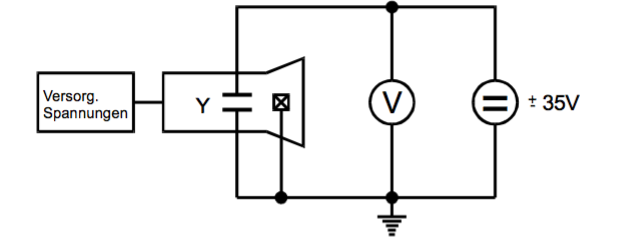
\includegraphics[height=5cm]{Schaltung1.png}
  \caption{Schaltung zur Untersuchung der Proportionalität \cite{skript1}.}
  \label{fig:schalt1}
\end{figure}
Um mittels der Methode des Kathodenstrahl-Oszillographen eine Sinusspannung
zu untersuchen, wird die Schaltung aus Abbildung \ref{fig:schalt2} verwendet.
\begin{figure}[H]
  \centering
  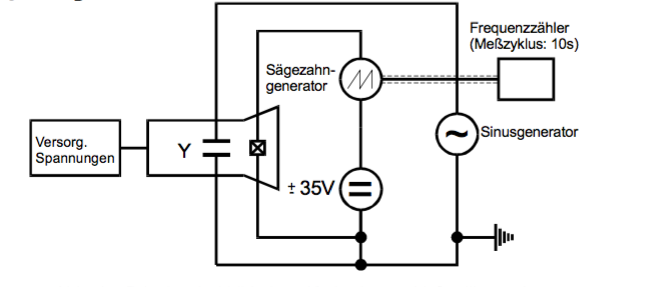
\includegraphics[height=5cm]{Schaltung2.png}
  \caption{Schaltung zur Untersuchung des Kathodenstrahl-Oszillographen \cite{skript1}.}
  \label{fig:schalt2}
\end{figure}
Zur Versuchsdurchführung wird die anglegte Sägezahnspannung solange variiert, bis
auf dem Leuchtschirm eine stehende Welle zu erkennen ist. Dies soll für verschiedene rationale
Verhältnisse der beiden Spannungen realisiert werden. Schlussendlich muss noch die maximale
Auslenkung durch die zu untersuchende Spannung ausgemessen werden.

\subsection{Ablenkung im magnetischen Feld}
Zur Untersuchung der Abhängigkeit der Verschiebung des Autreffpunktes von dem
magnetischen Feld wird eine Helmholtzspule verwendet, in deren Mitte das magnetische
Feld durch die Formel
\begin{equation}
  B = \mu_0 \frac{8}{\sqrt{125}}\frac{\text{I}\text{N}}{\text{R}}
  \label{eqn:helmholtz}
\end{equation}
gegeben ist, wobei $\mu_0 $ die magnetische Feldkonstante bezeichnet, I den Spulenstrom,
N die Windungszahl und R den Spulenradius.
Zunächst wird bei abgeschaltetem Magnetfeld
die Kathodenstrahlröhre in die Richtung der Horizontalkomponente ausgerichtet,
welche mit einem speziellen Kompass, dem sogenannten Deklinatorium-Inklinatorium ermittelt wurde.
Anschließend wird der Auftreffpunkt mittels Verschiebung durch elektrische Felder auf die
unterste Linie gelegt.
Nun wird bei Beschleunigungsspannungen von einmal $\SI{250}{\volt}$ und einmal $\SI{350}{\volt}$
die Helmholtzspule angeschaltet und der Spulenstrom und somit das Magnetfeld so
variiert, dass der Leuchtfleck jeweils auf den äquidistanten Linien liegt.


\noindent Zur Bestimmung des Erdmagnetfelds wird die Kathodenstrahlröhre zunächst
in Richtung der Nord-Süd-Achse ausgerichtet, welche erneut mit dem Deklinatorium-Inklinatorium
ermittelt wird. Der Auftreffpunkt wird dann notiert.
Nun wird die Kathodenstrahlröhre in Ost-West-Richtung ausgerichtet, sodass sich durch das
somit veränderte Magnetfeld eine Verschiebung ergibt, welche anschließend durch
ein mit der Helmholtzspule erzeugtes Gegenfeld genau wieder ausgeglichen wird.
Der hierzu verwendete Spulenstrom wird dabei notiert. Zuletzt muss noch mit dem
Deklinatorium-Inklinatorium der sogenannte Inklinationswinkel $\varphi$ bestimmt
werden.
